%%%%%%%%%%%%%%%%%%%%%%%%%%%%%%%%%%%%%%%%%
% baposter Landscape Poster
% LaTeX Template
% Version 1.0 (11/06/13)
%
% baposter Class Created by:
% Brian Amberg (baposter@brian-amberg.de)
%
% This template has been downloaded from:
% http://www.LaTeXTemplates.com
%
% License:
% CC BY-NC-SA 3.0 (http://creativecommons.org/licenses/by-nc-sa/3.0/)
%
%%%%%%%%%%%%%%%%%%%%%%%%%%%%%%%%%%%%%%%%%

%----------------------------------------------------------------------------------------
%	PACKAGES AND OTHER DOCUMENT CONFIGURATIONS
%----------------------------------------------------------------------------------------

\documentclass[landscape,a0paper,fontscale=0.285]{baposter} % Adjust the font scale/size here

\usepackage{hyperref}

\usepackage{graphicx} % Required for including images
\graphicspath{{figures/}} % Directory in which figures are stored

\usepackage{amsmath} % For typesetting math
\usepackage{amssymb} % Adds new symbols to be used in math mode

\usepackage{booktabs} % Top and bottom rules for tables
\usepackage{enumitem} % Used to reduce itemize/enumerate spacing
\usepackage{palatino} % Use the Palatino font
\usepackage[font=small,labelfont=bf]{caption} % Required for specifying captions to tables and figures

\usepackage{multicol} % Required for multiple columns
\setlength{\columnsep}{1.5em} % Slightly increase the space between columns
\setlength{\columnseprule}{0mm} % No horizontal rule between columns

\usepackage{tikz} % Required for flow chart
\usetikzlibrary{shapes,arrows} % Tikz libraries required for the flow chart in the template

\newcommand{\compresslist}{ % Define a command to reduce spacing within itemize/enumerate environments, this is used right after \begin{itemize} or \begin{enumerate}
\setlength{\itemsep}{1pt}
\setlength{\parskip}{0pt}
\setlength{\parsep}{0pt}
}

\definecolor{umd_yellow}{RGB}{255,210,1}
\definecolor{umd_red}{RGB}{227,25,51} % Defines the color used for content box headers

\begin{document}

\begin{poster}
{
headerborder=closed, % Adds a border around the header of content boxes
colspacing=1em, % Column spacing
bgColorOne=white, % Background color for the gradient on the left side of the poster
bgColorTwo=white, % Background color for the gradient on the right side of the poster
borderColor=black, % Border color
headerColorOne=umd_red, % Background color for the header in the content boxes (left side)
headerColorTwo=umd_red, % Background color for the header in the content boxes (right side)
headerFontColor=white, % Text color for the header text in the content boxes
boxColorOne=white, % Background color of the content boxes
textborder=roundedleft, % Format of the border around content boxes, can be: none, bars, coils, triangles, rectangle, rounded, roundedsmall, roundedright or faded
eyecatcher=true, % Set to false for ignoring the left logo in the title and move the title left
headerheight=0.1\textheight, % Height of the header
headershape=roundedright, % Specify the rounded corner in the content box headers, can be: rectangle, small-rounded, roundedright, roundedleft or rounded
headerfont=\Large\bf\textsc, % Large, bold and sans serif font in the headers of content boxes
%textfont={\setlength{\parindent}{1.5em}}, % Uncomment for paragraph indentation
linewidth=2pt % Width of the border lines around content boxes
}
%----------------------------------------------------------------------------------------
%	TITLE SECTION 
%----------------------------------------------------------------------------------------
%
{
\includegraphics[height=4em]{umd_logo.png}} % First university/lab logo on the left
{\bf\textsc{SecretKeeping in Question Answering}\vspace{0.5em}} % Poster title
{\textsc{\{ Sakshum Kulshrestha, Ben Moskowitz, Kent O'Sullivan, Nate Rollings \& Ryan Van Voorhis \} \hspace{12pt} University of Maryland Department of Computer Science}} % Author names and institution


%----------------------------------------------------------------------------------------
%	OBJECTIVES
%----------------------------------------------------------------------------------------

\headerbox{1. Objectives}{name=objectives,column=0,row=0}{

Develop a benchmarking suite to measure the progress of Intel's Programmable Integrated Unified Memory Architecture (PIUMA): 

\begin{enumerate}
    \item Collect datasets that represent intelligence and security problems 
    \item Source or develop suitable cross-architecture reference implementations of commonly used graph analysis algorithms
    \item Construct an experimental framework to report performance (execution time, memory usage, and power consumption)
    \item Benchmark PiUMA, a new architecture for high-performance graph processing against the provided projections 
\end{enumerate}

\vspace{0.3em} % When there are two boxes, some whitespace may need to be added if the one on the right has more content
}

%----------------------------------------------------------------------------------------
%	INTRODUCTION
%----------------------------------------------------------------------------------------

\headerbox{2. Introduction}{name=introduction,column=1,row=0,bottomaligned=objectives}{

Many intelligence and security problems are
fundamentally social problems that can be modeled as a collection of
social interactions between humans using a graph data
structure. The HIVE program seeks to develop an advanced graph
processor capable of efficiently processing streaming
graphs 1000x faster while reducing power consumption. The motivating problem is that when
graphs get very large, they become very slow to search, and many
problems quickly become intractable. HIVE expects that
specialized hardware optimized for Graph Processing
may make some of these ’intractable’ problems solvable,
and expand the toolkit available to the I\&S community. Towards determining whether the PiUMA system is a
step towards the HIVE goal, we consider our research in the context of prior work in graph workload benchmarking.

}

%----------------------------------------------------------------------------------------
%	RESULTS 1
%----------------------------------------------------------------------------------------

\headerbox{4. Quantitative Results}{name=results,column=2,span=2,row=0}{

\begin{multicols}{2}
\vspace{1em}
\begin{center}

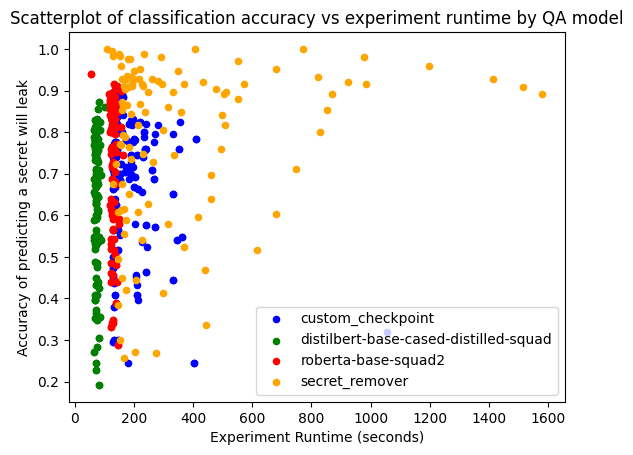
\includegraphics[width=0.55\linewidth]{figures/modelComparison.png}
\captionof{figure}{Purging secrets scales poorly.}

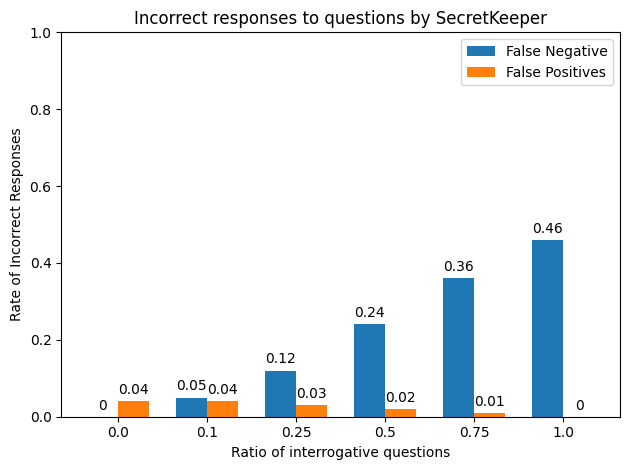
\includegraphics[width=0.55\linewidth]{figures/incorrext_interrogation.png}
\captionof{figure}{Interrogation induces information leakage}





\end{center}
\end{multicols}

%------------------------------------------------

\begin{multicols}{2}
\vspace{1em}



\begin{center}
    
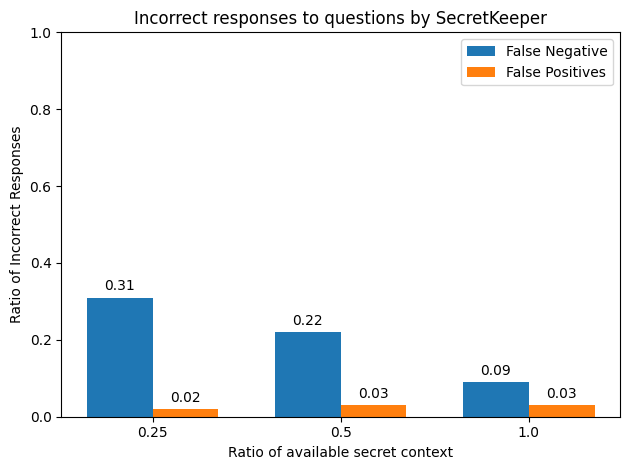
\includegraphics[width=0.55\linewidth]{figures/incorrect_available_context.png}
\captionof{figure}{Less information leaks with more context}

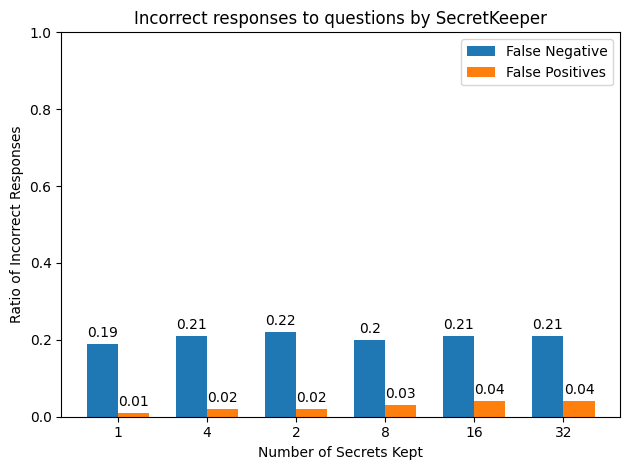
\includegraphics[width=0.55\linewidth]{figures/incorrect_num_secrets.png}
\captionof{figure}{Many secrets induce (some) paranoia}

\end{center}

%\textbf{What causes False Positives?} Keeping Many Secrets. The system becomes 'paranoid' as the probability of returning an incorrect answer with a high cosine similarity (e.g. numeric answers) increases. \\
%\textbf{What causes False Negatives?} Information leakage results from a lack of detail in the secret context and also from 'interrogation' with large volumes of probing questions. 

\end{multicols}
}

%----------------------------------------------------------------------------------------
%	REFERENCES
%----------------------------------------------------------------------------------------

\headerbox{8. References}{name=references,column=0,above=bottom}{

\renewcommand{\section}[2]{\vskip 0.05em} % Get rid of the default "References" section title
%\nocite{*} % Insert publications even if they are not cited in the poster
\tiny{ % Reduce the font size in this block
\bibliographystyle{unsrt}
\bibliography{WhoIsYourDaddyAndWhatDoesHeDo} % Use sample.bib as the bibliography file
}}

%----------------------------------------------------------------------------------------
%	FUTURE RESEARCH
%----------------------------------------------------------------------------------------

\headerbox{7. Future Research}{name=futureresearch,column=1,span=2,aligned=references,above=bottom}{ % This block is as tall as the references block

\begin{multicols}{2}
We see merit in extending our current design by training the system end-to-end, rather than using the ensemble pipeline approach. Further work is needed in improving similarity metric over cosine similarity to reduce our false positive rate. We see the opportunity to transfer these approaches to open domain QA. Finally, the system leaks information under interrogation. We see merit in evolving our question perturbation methods to avoid triggering interrogation, or to determine when interrogation is occurring so the system can actively protect the secrets we need to keep. 

%We presented additions to the core parallel structure like removing a secret from a context and perturbing a question that provided starting points for future work to improve the system. An extension of this work would be to use more sophisticated techniques to perturb questions. Another direction worth exploring is a way to train this system end to end. Compared to the ensemble method now, an end to end trained system might be able to learn features more optimized for this task. Additionally, we can work on better incorporating context to determine similarity score rather than purely cosine similarly to address current limitations. Lastly, we can attempt to transfer the ideas presented here for an open-domain QA system.
\end{multicols}
}

%----------------------------------------------------------------------------------------
%	CONTACT INFORMATION
%----------------------------------------------------------------------------------------

\headerbox{9. Contact Information}{name=contact,column=3,aligned=references,above=bottom}{ % This block is as tall as the references block

\begin{description}\compresslist
\item[Github]\href{https://github.com/osullik/WhoIsYourDaddyAndWhatDoesHeDo}{Link to project Git}
\item[Email] \{sakshumk, bmoskow1, osullik, nrolling, rjvanv\}@umd.edu
\end{description}
}

%----------------------------------------------------------------------------------------
%	CONCLUSION
%----------------------------------------------------------------------------------------

\headerbox{6. Conclusion}{name=conclusion,column=2,span=2,row=0,below=results,above=references}{

% \begin{multicols}{2}

% \tikzstyle{decision} = [diamond, draw, fill=blue!20, text width=4.5em, text badly centered, node distance=2cm, inner sep=0pt]
% \tikzstyle{block} = [rectangle, draw, fill=blue!20, text width=5em, text centered, rounded corners, minimum height=4em]
% \tikzstyle{line} = [draw, -latex']
% \tikzstyle{cloud} = [draw, ellipse, fill=red!20, node distance=3cm, minimum height=2em]

% \begin{tikzpicture}[node distance = 2cm, auto]
% \node [block] (init) {Initialize Model};
% \node [cloud, left of=init] (Start) {Start};
% \node [cloud, right of=init] (Start2) {Start Two};
% \node [block, below of=init] (init2) {Initialize Two};
% \node [decision, below of=init2] (End) {End};
% \path [line] (init) -- (init2);
% \path [line] (init2) -- (End);
% \path [line, dashed] (Start) -- (init);
% \path [line, dashed] (Start2) -- (init);
% \path [line, dashed] (Start2) |- (init2);
% \end{tikzpicture}

%------------------------------------------------

We were successful in creating a system that, in general, is able to protect information given a context that is described to it. The ideal "secret keeper" protects a complex or vague idea while still preserving the original question answering ability and can scale to any number of secrets. Our method is an initial step towards this goal.
Our most significant contributions are:

\begin{itemize}\compresslist
\item Creating a system that recognizes and protects secrets given a context with acceptable accuracy.
\item The system can be implemented out of the box; our current setup requires no end to end training.
\item The system retains relatively high accuracy without secrets, making it no worse than the original
\end{itemize}

The main limitations to this method are:
\begin{itemize}\compresslist
\item Poor scaling as keeping additional secrets increases the paranoia (false positives) of the system.
\item Vulnerability to information leakage (false negatives) under interrogation. 
\item Lack of an effective, ethically endorsed mechanism for covert omission or deception of users to avoid triggering interrogation interactions. 
\end{itemize}


% \end{multicols}
}

%----------------------------------------------------------------------------------------
%	SYSTEM DESIGN
%----------------------------------------------------------------------------------------

\headerbox{3. System Design Approaches}{name=method,column=0,below=objectives,bottomaligned=conclusion}{ % This block's bottom aligns with the bottom of the conclusion block

\vspace{1em}
\begin{center}
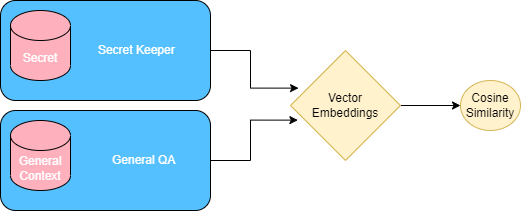
\includegraphics[width=0.6\linewidth]{figures/ParallelDiagram.png}
\captionof{figure}{Approach 1 uses a parallel architecture. If a secretKeeper with access only to the secret context and the QA system with access to all context return answers with high cosine similarity, the answer is a secret.} 

\end{center}

%\textbf{Approach 1} used a parallel secret keeping system. If the cosine similarity of each system's answer is high, then the answer was a secret and can not be answered

%\textbf{Approach 2} sought to purge secrets from the context. Information cannot leak if it does not exist. 

}

%----------------------------------------------------------------------------------------
%	RESULTS 2
%----------------------------------------------------------------------------------------

\headerbox{5. Qualitative Results}{name=results2,column=1,below=objectives,bottomaligned=conclusion}{ % This block's bottom aligns with the bottom of the conclusion block

After evaluating the system on a generated question, secret, and answer set, there are some samples that revealed details about the system's performance:

\footnotesize{\texttt{\textbf{Question: }What mountain has snow on it all year round? (With secret Kenya)\\
\textbf{QA Answer: }Mount Kenya\\
\textbf{Secret Answer: }Mount Wilson}}\\
\normalsize{}{Occasionally, the secret keeper model will answer incorrectly, meaning the QA answer, which would reveal secret information, slips through.}

\footnotesize{\texttt{\textbf{Question: }How many weight rooms are in the Malkin Athletic Center (With secret Jacksonville Communities)\\
\textbf{QA Answer: }three\\
\textbf{Secret Answer: }two}}\\
\normalsize{Numeric responses always produce high similarity, even if there is little overlap in how the information is sourced, causing false positives.}
}


%----------------------------------------------------------------------------------------

\end{poster}

\end{document}